\section{VoLTE音视频传输方案}
\label{chap:backinfo:volte}

%VoLTE实现概述

\insertFigure{
	\begin{figure}
		\centering
        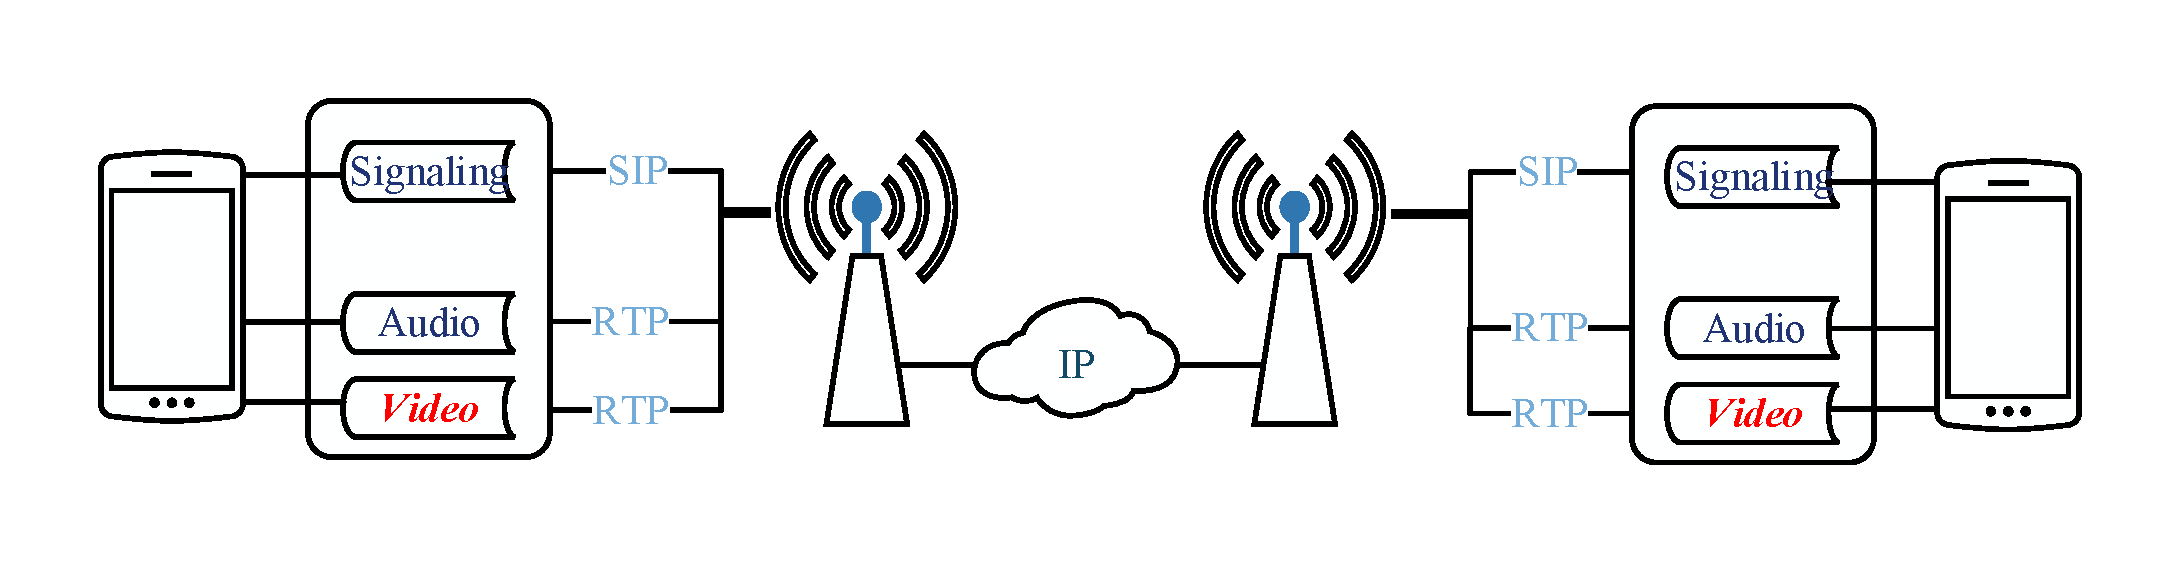
\includegraphics[width=0.95\textwidth]{chapters/chapter2/figures/volte-model.pdf}
        \caption{VoLTE视频通话中的数据流}\label{fig:2:volte-model}
	\end{figure}
}

语音通信功能是移动通信技术的最早需求,随着智能终端的发展,用户对数据传输的需求逐渐超越了对语音通信的需求。在移动通信标准中,基于LTE的第四代移动通信技术已经转变为全IP网络,实现了语音主导到数据主导的转换。不同于原有的通信方案,LTE优先对数据传输进行了优化,同时对音视频通话技术进行了支持。

\subsection{VoLTE数据处理流程}
\label{chap:backinfo:volte:datastream}

在2G及3G时代,基于电路交换音频通话技术,是支撑语音业务的核心解决方案。进入4G时代,全数据包交换的核心网络,无法兼容基于电路交换的音频通话,需要全新的解决方案。于是,基于VoIP音视频解决方案,基于LTE的VoLTE逐渐成为LTE网络中的主流。在实际应用中,支持VoLTE的终端能够快速建立呼叫,否则将回落到3G或2G网络,实现多种设备及场景之间的兼容。\nupcite{poikselka2012voice}

如图\nref{fig:2:volte-model},VoLTE视频通话过程中,需要建立的三个数据信道,分别为信令信道、语音信道及视频信道,所有的信道均采用数据包方式进行交互。通过音视频分离的方式,VoLTE实现了多场景兼容,通过信令信道,对通话的模式及参数进行协商,根据协商结果决定传输信道的模式及参数。相对2G及3G网络,LTE网络支持的数据上行速率有了显著提升,能够支撑更多的终端进行高清晰度的通话。\nupcite{ZHANG201929}

\insertTable{
    \begin{table}[]
        \centering
        \caption{LTE业务QCI分配表子表}
        \label{tab:2:qci-classification}
        \begin{threeparttable}
            \begin{tabular*}{\textwidth}{@{\extracolsep{\fill}}cccccc}
                \toprule
                QCI分类 & 资源类型 & 优先级 & 可接受延迟 & 可接受丢包率 & 服务类型 \\ 
                \midrule
                1 & 保证QoS & 2 & 100 ms & 0.01 & 语音通话 \\ 
                2 & 保证QoS & 4 & 150 ms & 0.001 & 视频通话 \\
                5 & 不保证QoS & 1 & 100 ms & 0.000001 & 信令 \\
                7 & 不保证QoS & 7 & 100 ms & 0.000001 & 交互式音视频 \\
                \bottomrule
            \end{tabular*}
            \begin{tablenotes}
                \footnotesize
                \item[] QoS指Quality of Service,服务质量
                \item[] QCI指Quality of Service Class Identifiers,QoS分类标签
            \end{tablenotes}
        \end{threeparttable}
    \end{table}
}

相较于固网,移动无线网络受噪声干扰明显,噪声会降低用户的通话体验,使得技术升级的效果减弱。如表\nref{tab:2:qci-classification},根据LTE业务分类,VoLTE的信令数据包具有1级最高优先级,可接受时延为100 ms,可接受丢包率为$10^{-6}$;VoLTE语音数据包具有2级优先级,可接受时延为100 ms,可接受丢包率为$10^{-2}$;VoLTE视频数据包优先级降为4级,可接受时延为150 ms,可接受丢包率为$10^{-3}$。另一方面,即使VoIP应用的数据包也是经LTE网络传输,其服务质量也是完全不同的,运营商网络只能保证尽力传输。VoIP的音视频数据对应的优先级为7,可接受时延为100 ms,可接受丢包率为$10_{-6}$。\nupcite{7154042,6996582,Li:2015:IVS:2810103.2813618}

因此,VoLTE相较其他通过LTE的VoIP应用,受网络调度产生抖动的概率要小,在构造时间隐通道过程中,修改余量较小,对时间隐通道的构建方法提出了挑战。

\subsection{VoLTE数据包传输特征}
\label{chap:backinfo:volte:packets}
%VoLTE音视频分流处理的模式(分清楚执行组件),结合传输的逻辑设计
在支持VoLTE的终端设备中,在视频通话过程中,参与数据处理的处理器通常由两部分组成。其中一个是AP(Application Processor)也就是应用处理器,另外一个是BP(Baseband Processor)也就是基带处理器。AP参与操作系统中通用数据的处理,BP负责的是无线通信数据的处理,二者相互补充,共同完成智能终端设备的数据处理任务。

\insertFigure{
	\begin{figure}
		\centering
        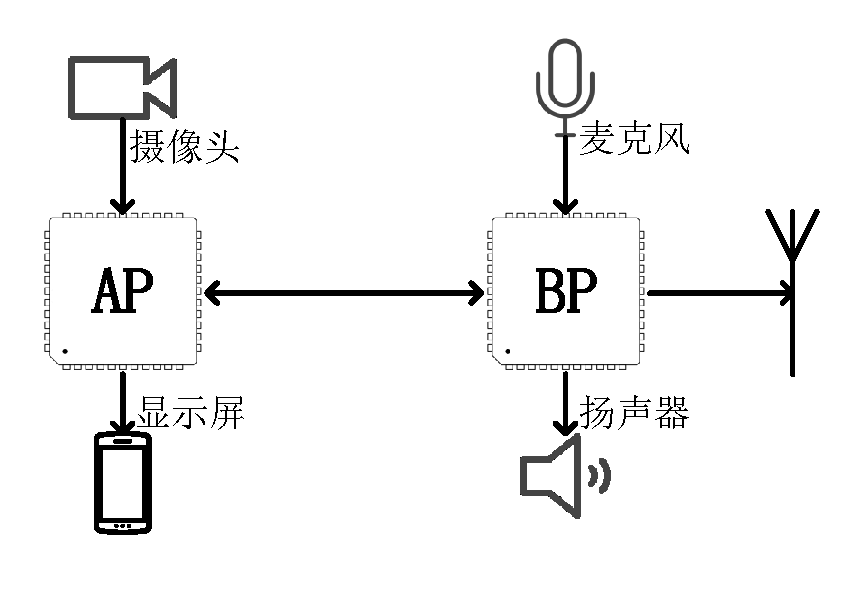
\includegraphics[width=0.55\textwidth]{chapters/chapter2/figures/ap-bp.pdf}
        \caption{VoLTE视频通话时AP与BP功能划分}\label{fig:2:ap-bp}
	\end{figure}
}

如图\nref{fig:2:ap-bp},在发送阶段,对于VoLTE语音数据来说,由基带处理器按照设定的时间间隔,完成模拟信号的采样、编码,并将打包好的语音数据包通过射频系统传输。对于VoLTE视频数据来说,由于图像处理模块集成到了应用处理器中,视频数据包的生成需要应用处理器参与。应用处理器调用摄像系统驱动,获取编码后的视频数据流,按照视频帧分别进行切分打包,得到RTP视频数据包,由系统内核中的协议栈进行发送处理。同样的,在接收阶段,VoLTE语音数据由基带处理器完成接收、解包、解码,并交由扬声器进行播放。VoLTE视频数据包则交付给系统中的网络组件,完成解包、解码后,调用显示组件显示在屏幕上。\nupcite{ZHANG201929,guo2019volte}

%抓包结果,分析传输特征,时间间隔、发送密度
\subsubsection{音视频数据包发送特征}
\label{chap:backinfo:volte:packets:send}
对于音频数据包来说,采用AMR-WB格式编码时,音频数据包在非静音期每20 ms发送一次,在静音期不发送数据包。\nupcite{8288828}对于视频数据包来说,数据包发送间隔取决于视频刷新率及编码结果,具有很大的不确定性。\nupcite{zhang2019timestamp}如图\nref{fig:2:audio-video},VoLTE视频数据包的长度虽然在1300字节左右有集中分布,但仍有部分数据包长度随机变化;VoLTE语音数据包的发送间隔具有规律性,但视频数据包在单个时间点聚集的现象更普遍。

\insertFigure{
	\begin{figure}
		\centering
        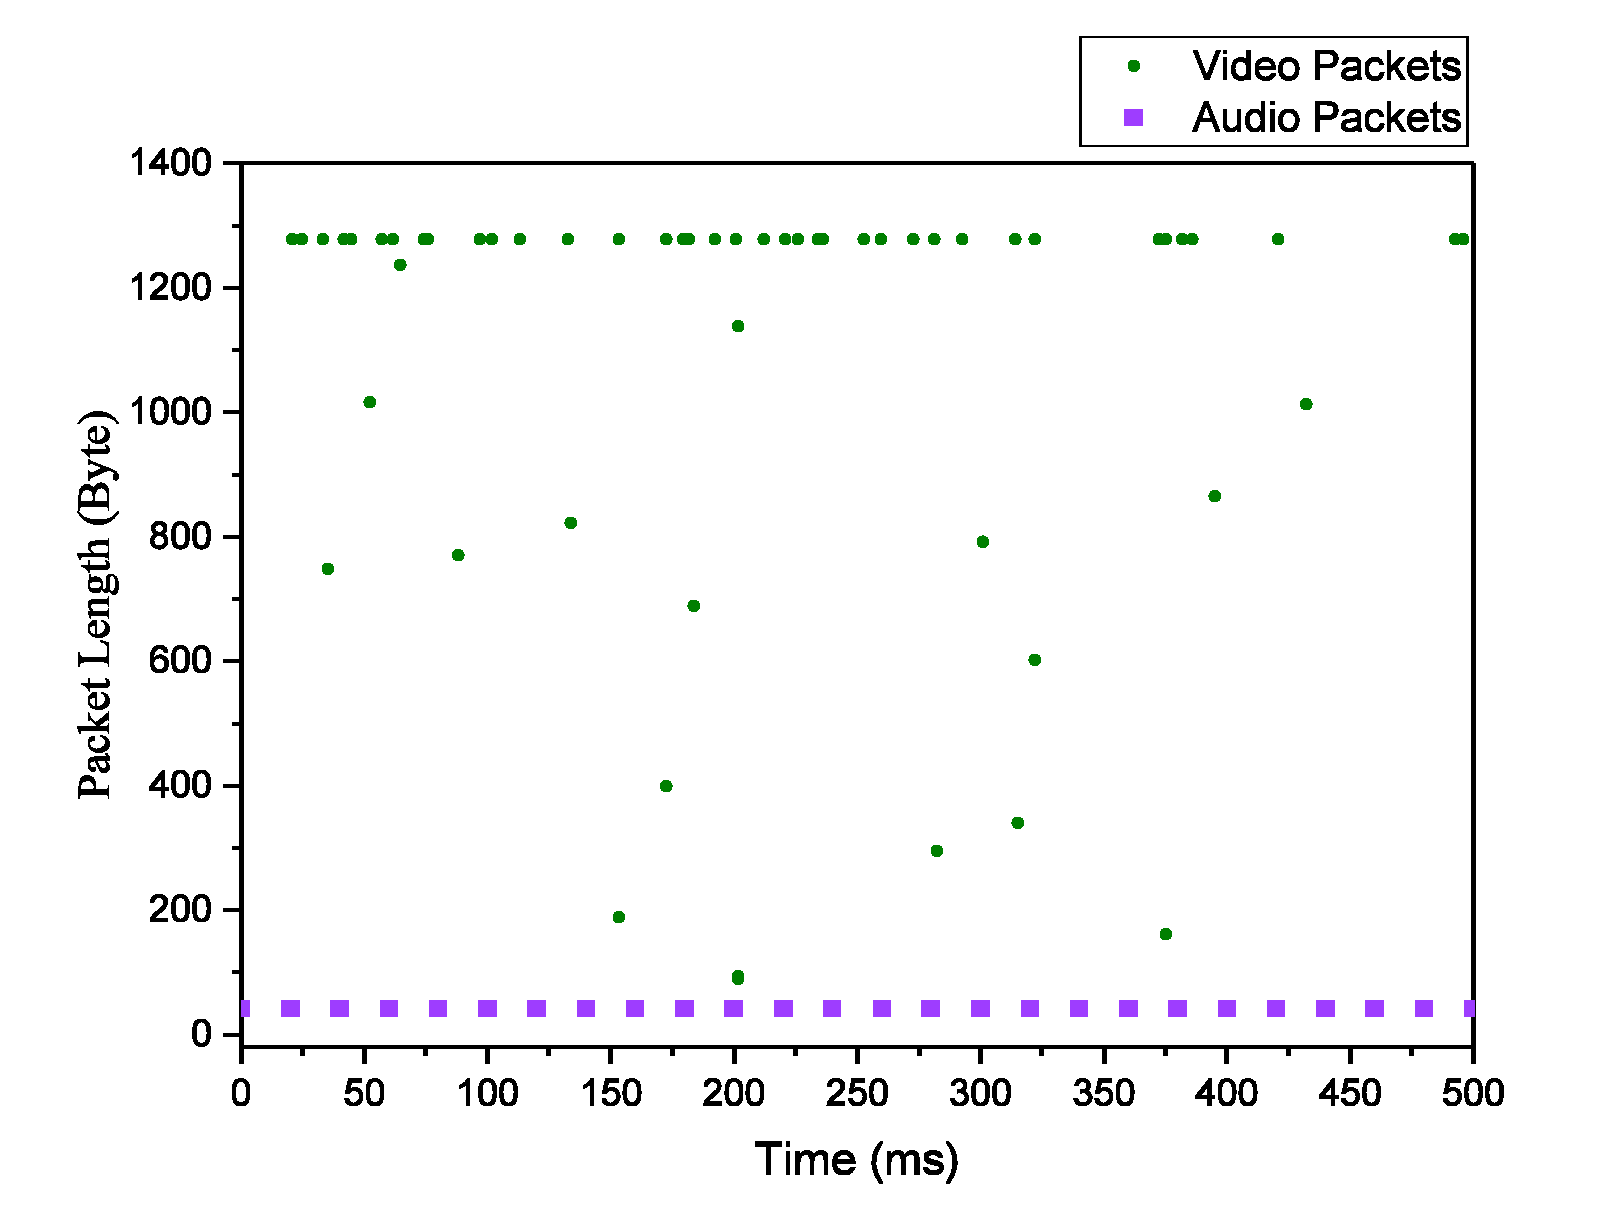
\includegraphics[width=0.8\textwidth]{chapters/chapter2/figures/ipds-audio-video.pdf}
        \caption{VoLTE音视频数据包发送间隔示意}\label{fig:2:audio-video}
	\end{figure}
}

\subsubsection{视频数据包发送与接收IPD分布特征}
\label{chap:backinfo:volte:packets:ipd}
如\nref{chap:backinfo:volte:packets:send}所述,VoLTE语音数据包的IPD规律性明显,对与语音数据包传输特征的控制,处产生可观测的异常分布。研究VoLTE视频数据包的传输特征,对VoLTE下时间隐通道构造方法的研究具有重要意义,VoLTE视频数据流对噪声敏感度低,便于时间隐通道隐匿在网络噪声中。

\insertFigure{
	\begin{figure}
		\centering
        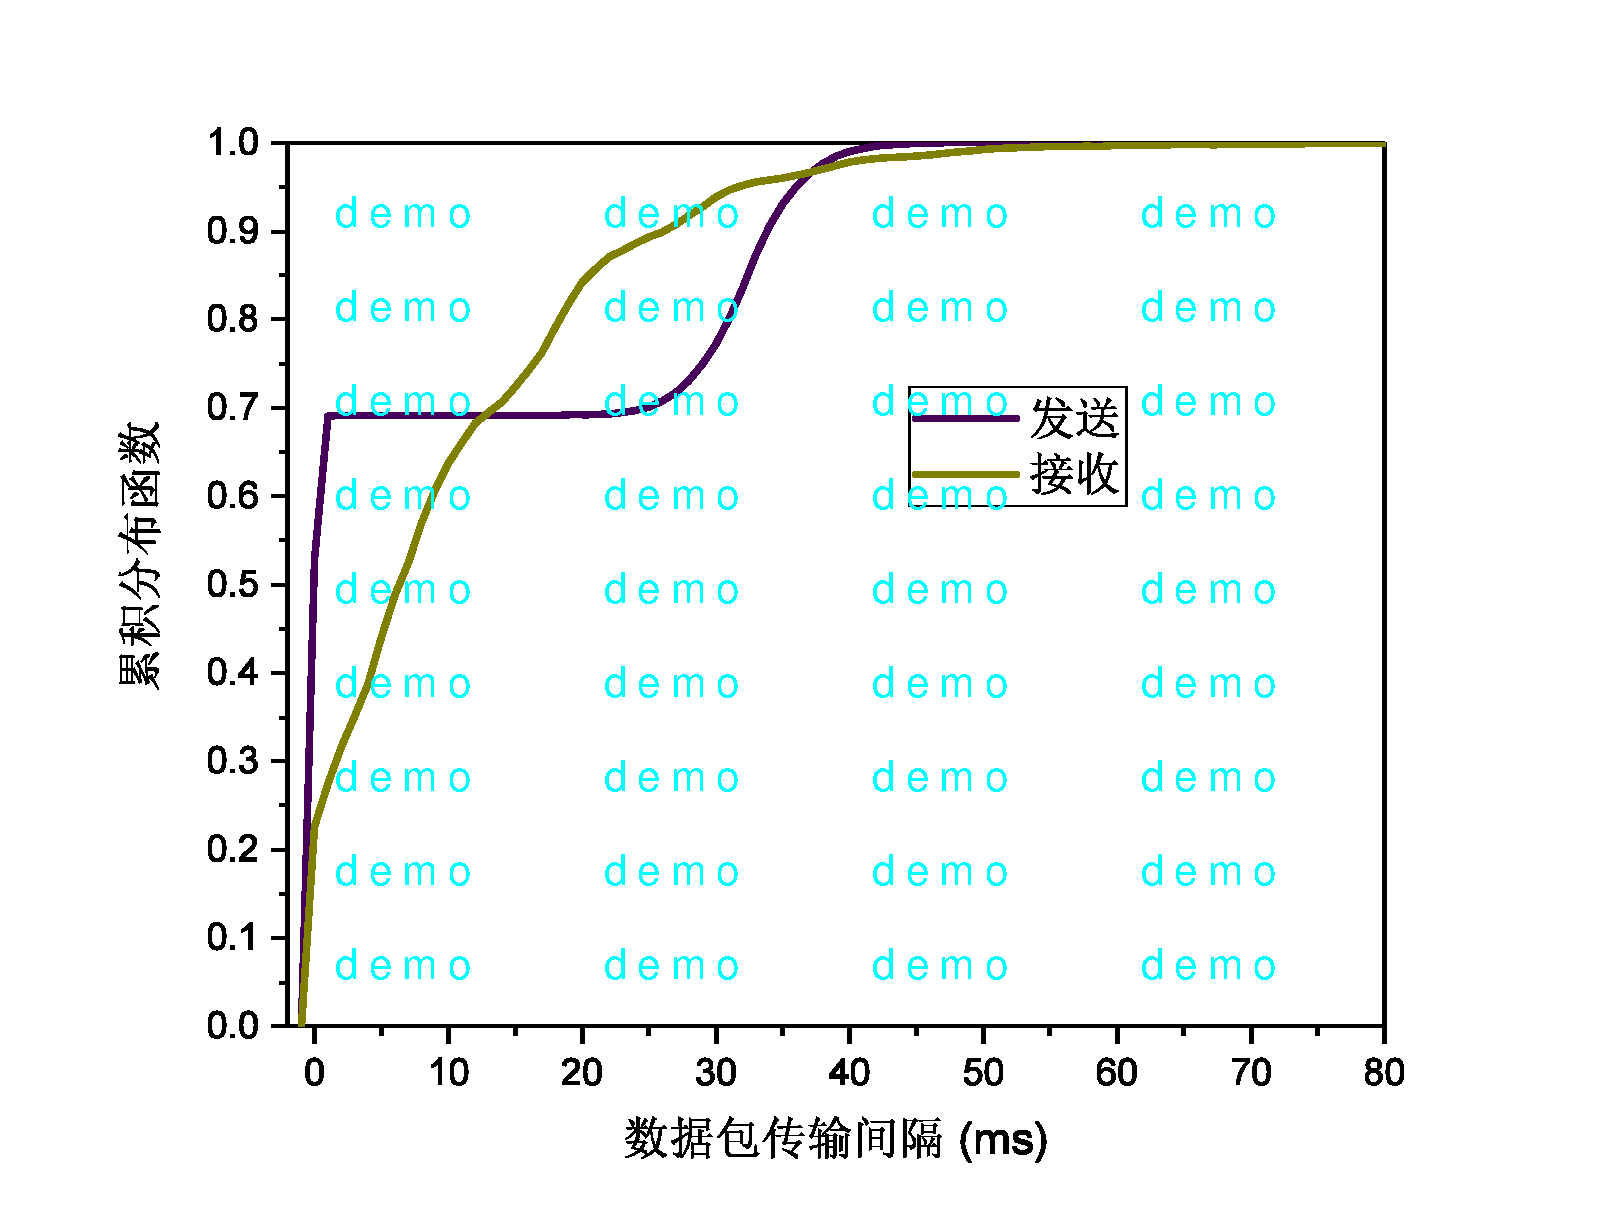
\includegraphics[width=0.8\textwidth]{chapters/chapter2/figures/cdf-send-receive.pdf}
        \caption{VoLTE视频数据包IPD的累积分布函数}\label{fig:2:cdf-ipd}
	\end{figure}
}

如图\nref{fig:2:cdf-ipd},在发送阶段,IPD主要集中在30 ms及0 ms两部分,由于视频刷新率为30 fps,每隔33 ms产生一个新的视频帧,而视频帧又有多个数据包组成,造成发送阶段CDF曲线不平滑。在接收阶段,受网络噪声及传输延迟的影响,IPD在$[0, 30]$区间之间集中分布,CDF曲线趋于平滑。因此,视频数据包在IPD方面,对时间隐通道的容忍性要优于语音数据包。

\subsubsection{VoLTE视频数据包丢包特征}
\label{chap:backinfo:volte:packets:dropout}
\insertFigure{
	\begin{figure}
		\centering
        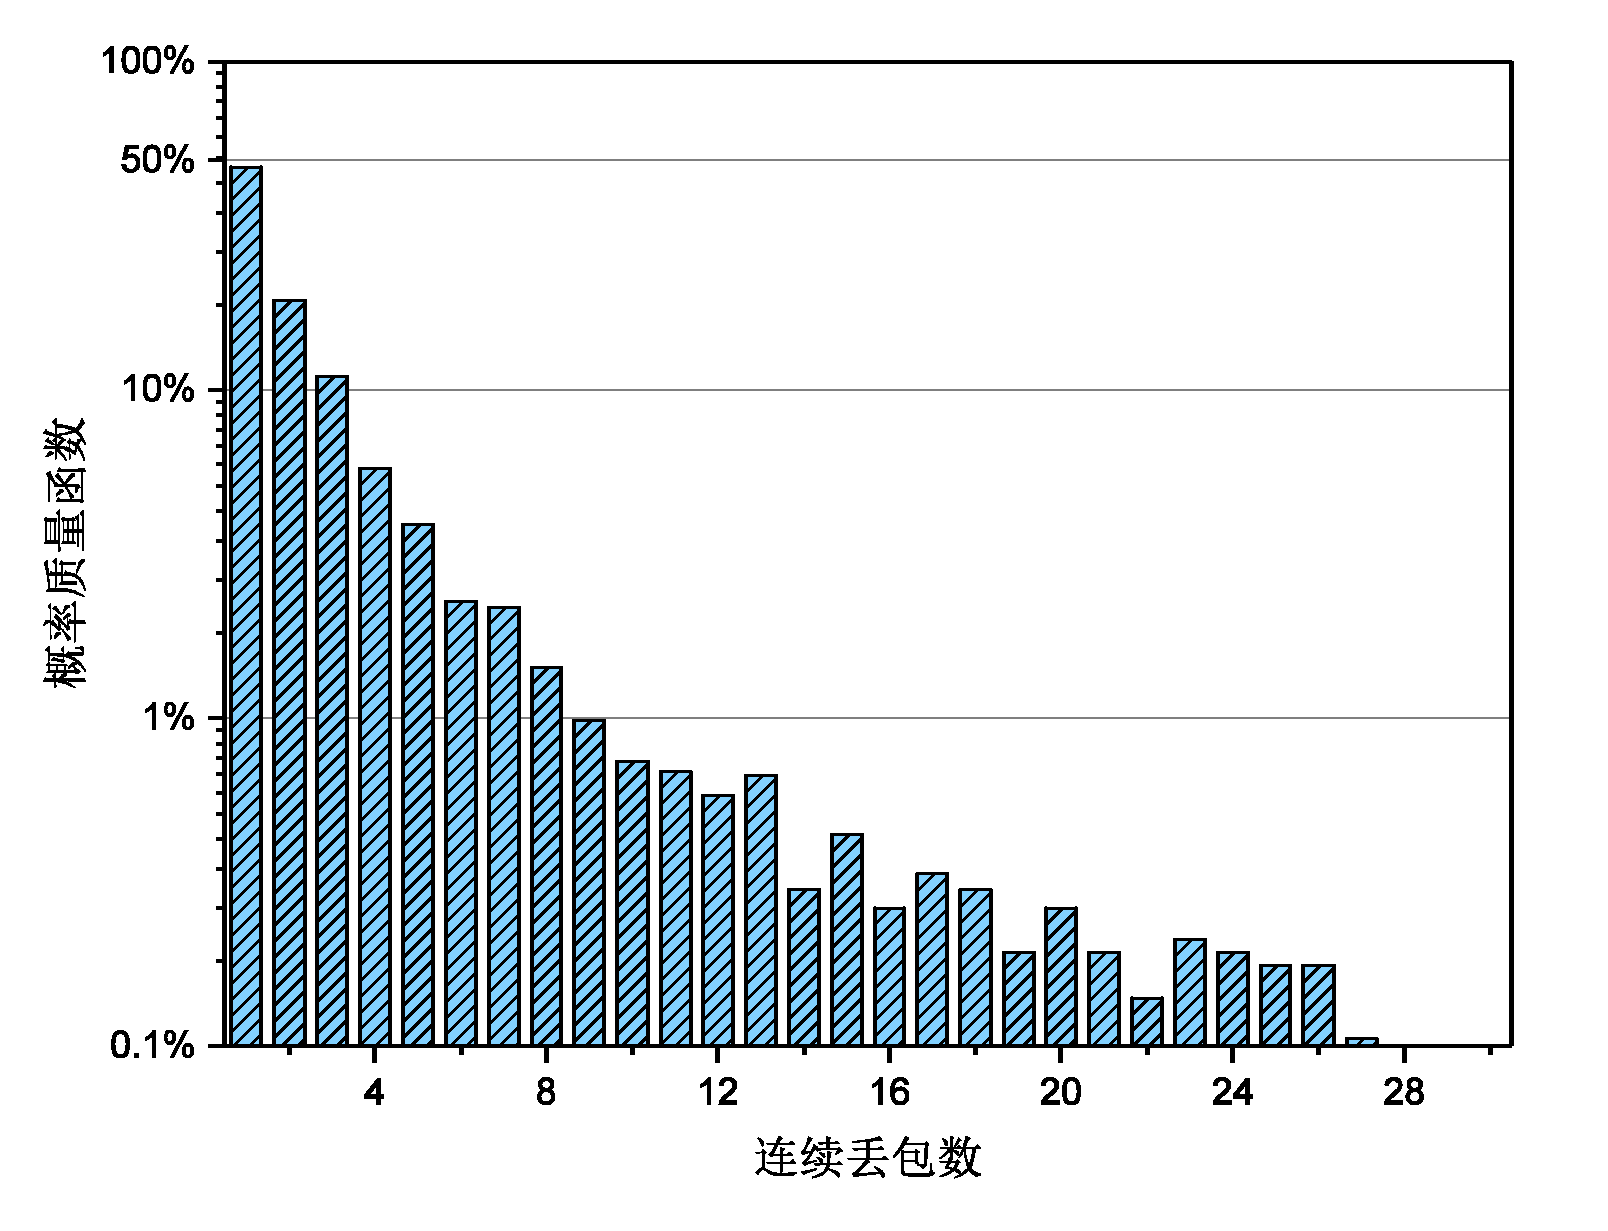
\includegraphics[width=0.8\textwidth]{chapters/chapter2/figures/pmf-dropout.pdf}
        \caption{连续丢包数量的概率密度函数}\label{fig:2:pmf-dropout}
	\end{figure}
}

对于VoLTE视频数据包,连续丢包数量的概率密度函数如图\nref{fig:2:pmf-dropout}。该统计结果,来自抓包得到的58万条VoLTE视频数据包,包含低噪声及高噪声在内的多种测试场景。PMF(Probability Mass Function)统计结果显示,VoLTE视频数据信道中的丢包事件,主要是单个数据包的离散丢包事件,大量的连续丢包事件占据的比例非常小。

\subsection{基于主动丢包的时间隐通道构造基础}
\label{chap:backinfo:volte:scheme}
VoLTE丢包的原因,主要发生在通信终端与基站的空口传输过程,在复杂的通信环境中,发送端与接收端均会出现丢包可能。对于监听者来说,只有监听了隐通道发送方的终端设备,才能监测到设备中的异常丢包事件。然而,在隐通道的威胁模型及实际应用中,监听方主要监听的是中间介质,基于主动丢包的时间有通道,符合一般的传输特征。

通过对VoLTE通话的理论及实际测试进行分析,在VoLTE场景中构建时间隐通道,尤其是通过主动丢包的方式构建时间隐通道,应当选择VoLTE视频信道作为宿主信道。与此同时,主动丢包的构建方式应当模拟离散丢包模式,并且在统计特征方面与已知统计结果拟合。另一方面,VoLTE视频信道自身的丢包率,已经超过了QCI的预期丢包率,证明当前VoLTE实现的优化,仍然不能完全保证不丢包,通过丢包方式构建时间隐通道可行。所以,本文选择VoLTE视频信道,作为时间隐通道的宿主信道。